%%%%%%%%%%%%%%%%%%%%%%%%%%%%%%%%%
%                               %
% Luther Michaels               % 
% ECE 351-52                    %
% Lab 5                         %
% October 7, 2021               %
% Step and Impulse Response     %
% of a RLC Band Pass Filter     %
%                Lab Report     %
%                               %
%%%%%%%%%%%%%%%%%%%%%%%%%%%%%%%%%

 

%%%%%%%%%%%%%%%%%%%%%%%%%%%%%%%%%%%%%%%%%%%
%%% DOCUMENT PREAMBLE %%%
\documentclass[12pt]{report}
\usepackage[english]{babel}
\usepackage{url}
\usepackage[utf8x]{inputenc}
\usepackage{amsmath}
\usepackage{graphicx}
\graphicspath{{images/}}
\usepackage{parskip}
\usepackage{fancyhdr}
\usepackage{vmargin}
\usepackage{listings}
\usepackage{hyperref}
\usepackage{xcolor}

\definecolor{codegreen}{rgb}{0,0.6,0}
\definecolor{codegray}{rgb}{0.5,0.5,0.5}
\definecolor{codeblue}{rgb}{0,0,0.95}
\definecolor{backcolour}{rgb}{0.95,0.95,0.92}

\lstdefinestyle{mystyle}{
	backgroundcolor=\color{backcolour},   
	commentstyle=\color{codegreen},
	keywordstyle=\color{codeblue},
	numberstyle=\tiny\color{codegray},
	stringstyle=\color{codegreen},
	basicstyle=\ttfamily\footnotesize,
	breakatwhitespace=false,         
	breaklines=true,                 
	captionpos=b,                    
	keepspaces=true,                 
	numbers=left,                    
	numbersep=5pt,                  
	showspaces=false,                
	showstringspaces=false,
	showtabs=false,                  
	tabsize=2
}

\lstset{style=mystyle}

\setmarginsrb{3 cm}{2.5 cm}{3 cm}{2.5 cm}{1 cm}{1.5 cm}{1 cm}{1.5 cm}

\title{5}	% Title						
\author{Luther Michaels}	% Author		
\date{October 7, 2021}   % Date

\makeatletter
\let\thetitle\@title
\let\theauthor\@author
\let\thedate\@date
\makeatother

\pagestyle{fancy}
\fancyhf{}
\rhead{\theauthor}
\lhead{\thetitle}
\cfoot{\thepage}
%%%%%%%%%%%%%%%%%%%%%%%%%%%%%%%%%%%%%%%%%%%%

\begin{document}
	
%%%%%%%%%%%%%%%%%%%%%%%%%%%%%%%%%%%%%%%%%%%%%%%%%%%%%%%%%%%%%%%%%%%%%%%%%%%%%%%%%%
%%% TITLE PAGE %%%
\begin{titlepage}
	\centering
	\vspace*{0.5 cm}
	
	\begin{center}    
		\textsc{\Large   ECE 351 - Section \#52}\\[2.0 cm]	
	\end{center}  
	\textsc{\Large Step and Impulse Response \\ of a RLC Band Pass Filter }\\[0.5 cm]
	\rule{\linewidth}{0.2 mm} \\[0.4 cm]
	{ \huge \bfseries \thetitle}\\
	\rule{\linewidth}{0.2 mm} \\[1.5 cm]
	\begin{minipage}{0.4\textwidth}
		\begin{flushleft} \large
		\end{flushleft}
	\end{minipage}~
	\begin{minipage}{0.4\textwidth}
		\begin{flushright} \large
			\emph{Submitted By:} \\
			Luther Michaels \break
			
			\emph{Submission Date:} \\
			October 7, 2021
		\end{flushright}
	\end{minipage}\\[2 cm]
\end{titlepage}
	
%%%%%%%%%%%%%%%%%%%%%%%%%%%%%%%%%%%%%%%%%%%%%%%%%%%%%%%%%%%%%%%%%%%%%%%%%%%%%%%%%%
%%% TABLE OF CONTENTS %%%
	
\tableofcontents
\pagebreak
	
%%%%%%%%%%%%%%%%%%%%%%%%%%%%%%%%%%%%%%%%%%%%%%%%%%%%%%%%%%%%%%%%%%%%%%%%%%%%%%%%%%
%%% LAB REPORT %%%
\renewcommand{\thesection}{\arabic{section}}
\section{Introduction}
	
The primary topics explored in this lab are impulse response and step response. Laplace transforms will be used to derive an s-domain transfer function describing a given RLC filter and its time-domain impulse response. The goal is to verify both this derived response and the step response found with the transfer equation using Python package operations. The end behavior of the step response can then be determined with the Final Value Theorem and confirmed with a Python plot. \\

This procedure utilizes the step function from our prior lab. Two functions from the numpy package that will be useful are numpy.abs, which obtains the magnitude of its input, and numpy.angle, which returns the phase. A technique for implementing a function is to represent the numerator and denominator in two separate matrices. Impulse and step functions can be determined from a transfer function input using scipy.signal.impulse and scipy.signal.step in Python.  All functions and plots can be produced using proper hand derivation and implementation via Python code written within the Spyder software. \\
	
\section{Equations}

\begin{equation*}
	u(t)=
	\begin{cases}
		0 & t < 0 \\
		1 & t \ge 0 \\
	\end{cases}
\end{equation*}
\begin{equation*}
	\mathcal{L}(u(t)) = u(s) = \frac{1}{s} \\
\end{equation*}
\begin{equation}
	H(s) = \frac{\frac{1}{RC}s}{s^2 + \frac{1}{RC}s + \frac{1}{LC}} \\
\end{equation}
\begin{equation*}
	y(t) = \frac{|g|}{\omega}e^{\alpha t}sin(\omega t + <g) \\
\end{equation*}
\begin{equation}
	h(t) = \frac{\sqrt{(-\frac{1}{2R^2C^2})^2 + (\frac{1}{2RC}\sqrt{\frac{4R^2C-L}{LR^2C^2}})^2}}{\frac{\sqrt{\frac{4R^2C-L}{LR^2C^2}}}{2}}e^{-\frac{1}{2RC}t}sin(\frac{\sqrt{\frac{4R^2C-L}{LR^2C^2}}}{2}t + (tan^{-1}(\frac{\sqrt{\frac{4R^2C-L}{LR^2C^2}}}{-\frac{1}{RC}}))u(t) \\ 
\end{equation}
\begin{equation*}
	\lim_{t\rightarrow \infty}\{h(t) * u(t)\} = 0 \\
\end{equation*}
	
\section{Methodology}

The necessary impulse and step response derivations for this lab were accomplished in the prelab. The first task, given in Part 1 of the lab manual, was to plot the the impulse response over the time interval from 0 to 1.2 ms. This required that Equation 2 first be implemented as a function in Python. The values for $ R $, $ L $, and $ C $ were defined outside of the function and passed as arguments. To keep the code clean, the individual parts of the equation were defined as variables $ p $, $ \alpha $, $ \omega $, $ |g| $, and $ <g $. The magnitude and phase of $ g $ were found using the numpy commands numpy.abs and numpy.angle. An extra $ + 0j $ term was included in each square root to inform Python to expect a complex result. These variables were then combined into the single sine function described by the general equation. \\

\begin{lstlisting}[language=Python]
""" Part 1, Task 1: HAND-CALCULATED IMPULSE RESPONSE """	
def h(t,R,L,C):   # additional R,L,C inputs  
	alpha = (-1 / (2 * R * C))
	omega = (1 / 2) * np.sqrt((1 / (R * C)) ** 2 - (4 * ((1/np.sqrt(L * C)) ** 2)) + 0 * 1j)
	p = alpha + omega  
	g = (1 / (R * C)) * p 
	g_mag = np.abs(g)        # magnitude
	g_phase = np.angle(g)    # phase
	h = (((g_mag) / np.abs(omega)) * np.exp(alpha * t) * 	np.sin((np.abs(omega) * t) + g_phase)) * u(t)
	return h
\end{lstlisting}

As in prior experiments, the time interval was set to [0, 1.2 ms] using numpy.arange. The function was plotted using standard matplotlib.pyplot commands to format the chart, generating both a title and axis labels. The step size had to be lowered to $ 1 \times 10^{-5} $ in order to properly view the plot shape with good resolution. \\

In Task 2 of Part 1, the impulse response was requested using the scipy Python package to verify the result of Task 1. After copying the step function from Lab 2, Equation 1 was implemented in two matrices for the numerator and denominator. Each matrix contained the three coefficients present (including zeros as needed). These two matrices were entered into the function scipy.signal.impulse, returning an output with its associated time variable. These two were then plotted to produce the impulse response which was included as a subplot to that of Task 1. \\

Part 2 began with the task of plotting the step response via scipy from 0 to 1.2 ms. This response also used the transfer function. The matrix variables from Task 2 of Part 1 were input into the function scipy.signal.step. The two outputs were plotted to form a single graph of the step response. Task 2 requested the Final Value Theorem be used on the step response in the s-domain to determine by hand the end behavior of the function. This derivation is shown below. The discussion of the results prescribed by Task 3 will be included in the Results section. 

\begin{equation*}
	H(s) = \frac{\frac{1}{RC}s}{s^2 + \frac{1}{RC}s + \frac{1}{LC}}
\end{equation*}
\begin{equation*}
	u(s) = \frac{1}{s}
\end{equation*}
\begin{align*}
	F(s) &= H(s)u(s) \\
	&= \frac{\frac{1}{RC}}{s^2 + \frac{1}{RC}s + \frac{1}{LC}} \\
	sF(s) &= s(H(s)u(s)) \\
	&= \frac{\frac{1}{RC}s}{s^2 + \frac{1}{RC}s + \frac{1}{LC}}
\end{align*}
\begin{align*}
	\lim_{t\rightarrow \infty}\{f(t)\} &= \lim_{s\rightarrow 0}\{sF(s)\} \\
	\lim_{t\rightarrow \infty}\{h(t) * u(t)\} &= \lim_{s\rightarrow 0}\{\frac{\frac{1}{RC}s}{s^2 + \frac{1}{RC}s + \frac{1}{LC}}\} \\
	&= \frac{\frac{1}{RC}(0)}{(0)^2 + \frac{1}{RC}(0) + \frac{1}{LC}} \\
	&= 0
\end{align*}
Github Link: \url{https://github.com/Luther-Michaels} \\
	
\section{Results}

The plots for the hand-calculated impulse response function and the impulse response computed with scipy.signal are shown in the top and bottom subplots respectively of the below figure. Each is properly displayed over the time interval from 0 to 1.2 ms. Given that both subplots show a sinusoidal decay as prescribed by Equation 2, our intuition would support their validity. This is further evidenced by the fact that the plots are identical with matching axes, despite the different methods. The values of the y-axis are also to be expected given the values of $ R $, $ L $, and $ C $. The step size has been set properly for good resolution. \\ 

\begin{center}
	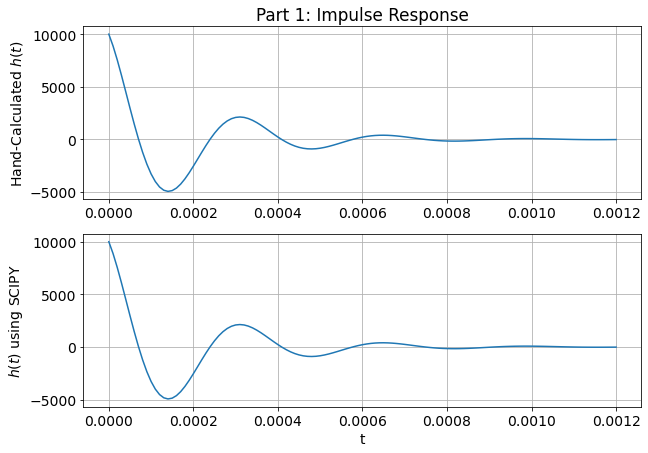
\includegraphics[scale = 0.495]{Lab 5 - Plots/Part1.png}\\[1.0 cm]
\end{center}

The step response obtained using scipy.signal.step on Equation 1, the transfer function, is provided in the following plot. The time interval has been properly preserved over 0 to 1.2 ms. The fact that the function features sinusoidal decay like the impulse response also matches our expectation. Given this decay, it is evident that the end behavior of the function as time reaches towards infinity is a steady approach towards zero. \\

\begin{center}
	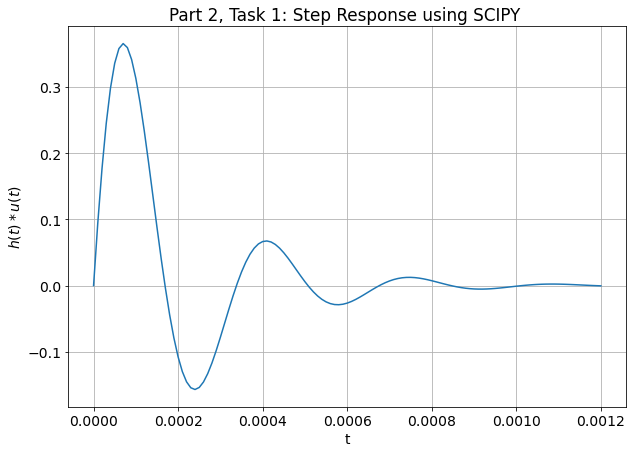
\includegraphics[scale = 0.495]{Lab 5 - Plots/Part2-Task1.png}\\[1.0 cm]
\end{center}

The results of this plot align closely with those indicated by using the Final Value Theorem on the step response. As shown in the equation below, the step response approaches zero as time goes to infinity. This assertion makes sense considering the sinusoidal decay present in the function outcome. It also makes sense because the endpoint must reach towards zero for a system to be stable. This stability is supported by the RLC circuit's transfer function.

\begin{equation*}
	\lim_{t\rightarrow \infty}\{h(t) * u(t)\} = 0
\end{equation*} \\
	
\section{Error Analysis}
	
The main source of difficulty I had with this lab was the step size. My step size was originally set to $ 1 \times 10^{-3} $ as in the prior labs. With this size, however, the plots did not obtain enough detailed points to accurately represent the shape I expected. At first, I reviewed my hand-calculated impulse response function definition to find the error. In the process I made my code much more clean and readable, but could not find the problem. The solution was only found after searching through the code thoroughly. With the TA's assistance, I discovered that the step size was too large and decreased it to $ 1 \times 10^{-5} $. \\  

My derivation of the phase for Equation 2 was also incorrect at first. I discovered this during the TA's demo of the prelab solution. To fix the problem, I swapped the numerator and denominator of my arctangent function which I had flipped. \\
	
\section{Questions}

1. The Final Value Theorem from Part 2 Task 2 indicated that the step response would approach zero as time went towards infinity. Our physical circuit components for this RLC bandpass filter include the resistor, inductor, and capacitor. As a step input is provided, the capacitor charges and discharges through the resistor and inductor. These two components slowly drain the input. Consequently, with each recharge of the capacitor a lower peak value is attainable until it eventually hits zero. \\

2. The lab tasks, expectations, and deliverables were all communicated clearly. \\
	
\section{Conclusion}

This lab grew our familiarity with impulse and step functions, developed our skills in deriving equations directly from circuitry, and solidified our understanding of the Final Value Theorem. We learned a new way to implement functions in Python as well as methods to keep our code clean and readable. \\

If this lab were repeated, I would have the students compute the time-domain step response by hand, implement it as a function in Python, plot it, and compare with the other plot. This would allow verification of this response result in addition to the impulse response. In this lab I learned the importance of always checking that the step size is adequate for good plot resolution. I was also reminded of the value in producing generalized solutions to equation derivations. These lessons will be useful in future work in resolving apparent plot errors and deriving necessary lab equations. \\
	
\newpage
\begin{thebibliography}{111}
		
	\bibitem{S}
Sullivan, Dennis M. (2018) {\it  Signals and Systems for Electrical Engineers I}. Nevada: CreateSpace Independent Publishing Platform.
		
\end{thebibliography}
\end{document}

% Lab Report based on template created by Roza Aceska.